\chapter{闭弦、能级匹配与对偶性}

\lectureoverview{闭弦在其两个内禀方向上支持彼此独立的波。对这些波作量子化，乍看之下似乎会使开弦的光子加倍，但弦坐标原点平移下的不变性消去了那些单侧状态。第一个存活下来的能级包含一个无质量的自旋二粒子。随后，改变描述方式这一同样的想法引出了一个更广泛的问题：当耦合常数变化时，说某个对象是基本的究竟意味着什么？}

\section{一个被留作备用的生成元}

在画出闭弦之前，让我们从正则力学中回顾一个事实。设
\begin{equation}
  L=L(q_i,\dot q_i),
\end{equation}
并定义与\(q_i\)共轭的动量为
\begin{equation}
  p_i=\frac{\partial L}{\partial\dot q_i}.
\end{equation}
一个无穷小连续变换可以写成
\begin{equation}
  \delta q_i=\epsilon f_i(q),
  \label{eq:l04-infinitesimal-transformation}
\end{equation}
其中\(\epsilon\)是一个小参数。若该变换是一个对称性，诺特定理便给出一个守恒荷。将坐标位移除以公共参数，即得生成元
\begin{equation}
  Q=\sum_i p_i f_i(q)
   =\frac{1}{\epsilon}\sum_i p_i\,\delta q_i.
  \label{eq:l04-noether-charge}
\end{equation}
在量子力学中，\(Q\)就是生成相应小变换的算符。

\(xy\)平面内的旋转是熟悉的例子。取一种取向选择，
\begin{equation}
  \delta x=\epsilon y,
  \qquad
  \delta y=-\epsilon x,
\end{equation}
而\eqref{eq:l04-noether-charge}就成为角动量，至多相差同一个符号选择。这个具体例子并不重要。重要的是那个模式：动量与无穷小位移缩并便给出生成元。

\begin{figure}[H]
  \centering
  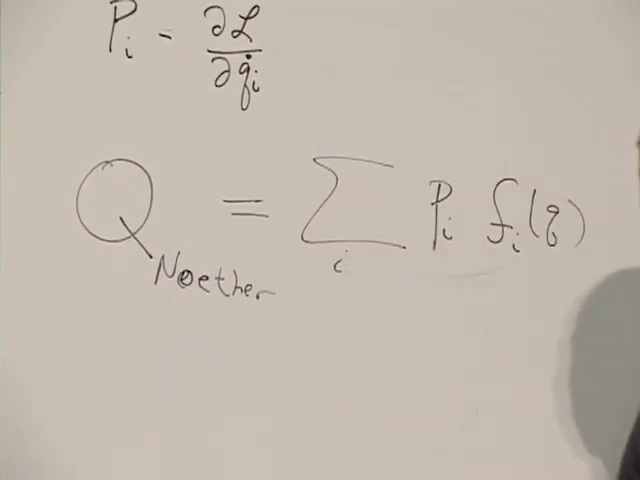
\includegraphics[width=0.76\textwidth]{lecture_04_figure_01.png}
  \caption{为闭弦坐标的后续平移而保留的正则动量与诺特生成元。}
  \lectureframe{00:05:00}
  \label{fig:l04-noether-board}
\end{figure}

我们不久将遇到一个对称性，其坐标不是普通空间中的点，而是弦上各点的标记。式\eqref{eq:l04-noether-charge}正是为此而被置于手边。

\section{环绕一圈的坐标}

闭弦没有端点。选取一个参数
\begin{equation}
  0\leq \sigma<2\pi
\end{equation}
并暂且把某一点标记为\(\sigma=0\)。绕行一半处是\(\sigma=\pi\)；四分之一圈和四分之三圈分别是\(\pi/2\)和\(3\pi/2\)。这个标记确立的是一种坐标约定，尚不是物理特征。

\begin{figure}[H]
  \centering
  \begin{minipage}[t]{0.58\textwidth}
    \centering
    \includegraphics[width=\textwidth]{lecture_04_figure_02.png}
    \par\smallskip\footnotesize (a) 黑板上的带标记的圈。
  \end{minipage}\hfill
  \begin{minipage}[t]{0.37\textwidth}
    \centering
    \begin{adjustbox}{max width=\linewidth}
    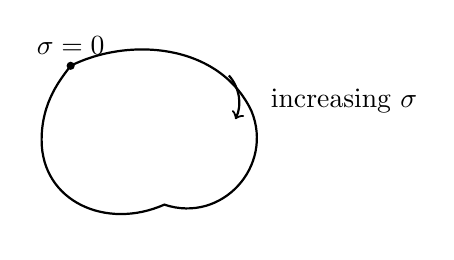
\begin{tikzpicture}[scale=0.82]
      \draw[thick]
        (0.1,1.1)
        .. controls (1.0,1.55) and (2.4,1.45) .. (2.9,0.4)
        .. controls (3.25,-0.45) and (2.45,-1.35) .. (1.55,-1.05)
        .. controls (0.65,-1.45) and (-0.35,-1.0) .. (-0.35,-0.05)
        .. controls (-0.35,0.55) and (-0.05,0.9) .. (0.1,1.1);
      \fill (0.1,1.1) circle (1.8pt);
      \node[above] at (0.1,1.12) {\(\sigma=0\)};
      \draw[->,thick] (2.55,0.95) arc[start angle=42,end angle=-25,radius=0.62];
      \node[right] at (3.05,0.55) {increasing \(\sigma\)};
    \end{tikzpicture}
    \end{adjustbox}
    \par\smallskip\footnotesize (b) 内禀取向。
  \end{minipage}
  \caption{标记一个点以定义原点，箭头则固定\(\sigma\)增大的方向。}
  \lectureframe{00:06:48}
  \label{fig:l04-closed-string-origin}
\end{figure}

沿圈的箭头是一种\emph{内禀}取向。切不可把它与\(xy\)平面内的顺时针或逆时针运动相混淆。想象一条带标记的橡皮筋从黑板上被提起、翻面，再放回去。它表观的顺时针方向反转了，而其内禀标记的次序并未反转。\(\sigma\)增大仍然是\(\sigma\)增大。

这一区分支配着右行波与左行波的语言。在本章中，右行扰动指的是朝\(\sigma\)增大的方向传播的扰动，左行扰动指的是朝\(\sigma\)减小的方向传播的扰动。这两个名称都没有告诉我们该扰动在房间里看起来朝哪个方向运动。

取向在最初的强子弦图像中曾起过具体作用。断开一根有取向的流管，会在一端产生一个夸克，在另一端产生一个反夸克；内禀箭头区分了这两端。人们也可以构造无取向的弦理论，但在目前的讨论中，我们保留箭头以及沿它的两个方向。

\section{周期性条件与行波}

设\(X(\sigma,\tau)\)和\(Y(\sigma,\tau)\)为弦的两个横向坐标，\(\tau\)表示时间。若还存在额外的横向坐标，其处理方式完全相同。由于\(\sigma=0\)和\(\sigma=2\pi\)标记的是同一个点，
\begin{equation}
  X(\sigma+2\pi,\tau)=X(\sigma,\tau),
  \qquad
  Y(\sigma+2\pi,\tau)=Y(\sigma,\tau).
  \label{eq:l04-periodicity}
\end{equation}

\begin{figure}[H]
  \centering
  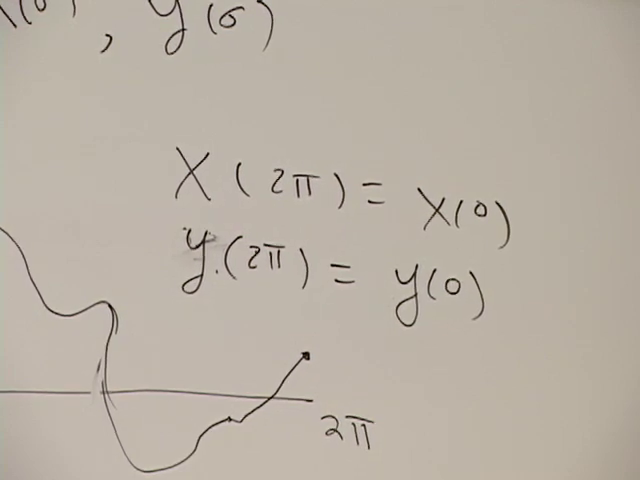
\includegraphics[width=0.76\textwidth]{lecture_04_figure_03.png}
  \caption{两个横向坐标的周期性边界条件。}
  \lectureframe{00:12:40}
  \label{fig:l04-periodicity-board}
\end{figure}

因此，一个局域化的抖动可以无限期地循环传播。当它到达\(2\pi\)时，它就直接在\(0\)处重新出现。这与开弦不同：在开弦上，行波到达端点后会反射；原本左行的变成右行，反之亦然。驻波对开弦来说是自然的，而闭弦则容许两个独立传播的波族。

\subsection{复傅里叶模式}

周期函数的一个便利基是
\begin{equation}
  e^{in\sigma}=\cos(n\sigma)+i\sin(n\sigma),
  \qquad n\in\mathbb Z.
\end{equation}
整数条件由周期性强制给出：
\(e^{in(\sigma+2\pi)}=e^{in\sigma}\)。例如，若把\(n\)替换为半整数，则绕行一周后函数就会改变。

暂时略去时间依赖，黑板上的展开式为
\begin{align}
  X(\sigma)
  &=
  X_0+
  \sum_{n>0}X_n e^{in\sigma}
  +\sum_{n>0}X_{-n}e^{-in\sigma},
  \label{eq:l04-fourier-x}\\
  Y(\sigma)
  &=
  Y_0+
  \sum_{n>0}Y_n e^{in\sigma}
  +\sum_{n>0}Y_{-n}e^{-in\sigma}.
  \label{eq:l04-fourier-y}
\end{align}
对于实的\(X\)和\(Y\)，在经典层面上，负指标系数是正指标系数的复共轭。零模\(X_0\)和\(Y_0\)确定质心位置；它们是位置，而不是内部振动。

\begin{figure}[H]
  \centering
  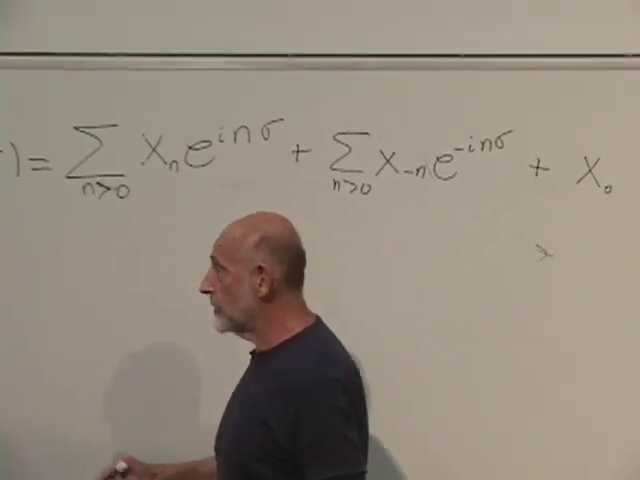
\includegraphics[width=0.82\textwidth]{lecture_04_figure_04.png}
  \caption{周期傅里叶展开的正指标部分与负指标部分，随后是零模。}
  \lectureframe{00:20:00}
  \label{fig:l04-fourier-board}
\end{figure}

\begin{classroomqa}
\audiencequestion{如果这些是行波，那么时间坐标在哪里？\lecturetimestamp{00:19:05}}
\lecturerresponse{它只是在黑板记号中被略去了。行波解携带一个同时涉及\(\sigma\)和\(\tau\)的相位。按照下文所用的约定，一族有
\(e^{-in(\tau-\sigma)}\)，另一族有
\(e^{-in(\tau+\sigma)}\)。}
\end{classroomqa}

因此，决定传播的是完整的相位，而不是单纯空间傅里叶因子中\(n\)的符号本身。我们可以写出
\begin{equation}
  X(\sigma,\tau)=X_R(\tau-\sigma)+X_L(\tau+\sigma),
  \label{eq:l04-chiral-solution}
\end{equation}
对\(Y\)也类似。哪一族被称为\(R\)而不是\(L\)只是一个约定；不变的事实是，沿\(\sigma\)圆有两个相反方向。\editorialnote{某一瞬间的因子\(e^{in\sigma}\)本身并不指定一个行波。只有在给定时间相位之后，传播才被确定。}

\section{两个方向上的能量}

局域动力学与开弦相同。在这里所用的简化归一化下，
\begin{equation}
  L\propto
  \int_0^{2\pi}d\sigma\,
  \left[
    \dot X^2-X'^2+\dot Y^2-Y'^2
  \right],
  \label{eq:l04-string-lagrangian}
\end{equation}
其中点表示\(\partial_\tau\)，撇表示
\(\partial_\sigma\)。能量在动能项与弹性项之间取正号：
\begin{equation}
  E\propto
  \int_0^{2\pi}d\sigma\,
  \left[
    \dot X^2+X'^2+\dot Y^2+Y'^2
  \right].
  \label{eq:l04-string-energy}
\end{equation}
对任一横向坐标，
\begin{equation}
  \dot X^2+X'^2
  =
  \frac12(\dot X+X')^2+
  \frac12(\dot X-X')^2.
  \label{eq:l04-energy-square-completion}
\end{equation}
交叉项相消，恰好留下原来的动能与梯度能量。

\begin{figure}[H]
  \centering
  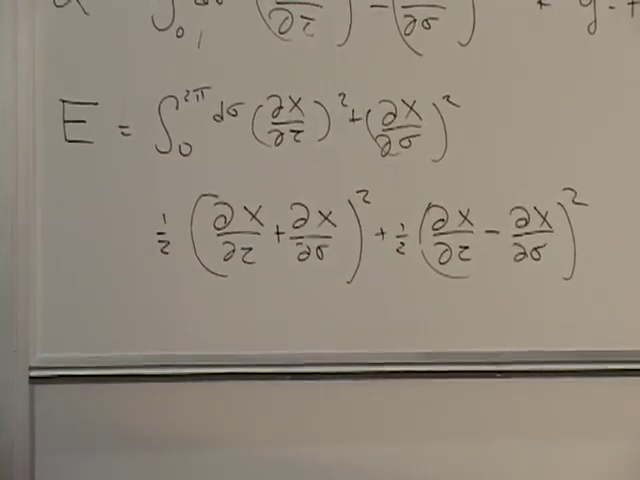
\includegraphics[width=0.82\textwidth]{lecture_04_figure_05.png}
  \caption{总能量被重新组织到两个行波扇区中。}
  \lectureframe{00:25:10}
  \label{fig:l04-energy-board}
\end{figure}

对于\(X_R(\tau-\sigma)\)，有\(\dot X_R=-X_R'\)；对于
\(X_L(\tau+\sigma)\)，有\(\dot X_L=X_L'\)。因此，\eqref{eq:l04-energy-square-completion}中的两个平方项分离出两个手征族。包括每一个横向坐标，定义
\begin{align}
  E_L&\propto
  \frac12\int_0^{2\pi}d\sigma
  \sum_I(\dot X^I+X^{I\prime})^2,\\
  E_R&\propto
  \frac12\int_0^{2\pi}d\sigma
  \sum_I(\dot X^I-X^{I\prime})^2.
  \label{eq:l04-left-right-energies}
\end{align}
于是\(E=E_L+E_R\)。由于在这一阶段方程是线性的，来自两个扇区的波彼此穿过而不发生散射。

\subsection{两倍的振子数}

把傅里叶级数代入
\eqref{eq:l04-string-lagrangian}，会把每个非零模系数变成一个谐振子。其频率正比于\(|n|\)：波长越短，频率越高，因此激发能越大。与开弦不同，每个正频率都以两个独立传播的副本出现。

黑板上把\(X\)极化的产生算符标为
\(a_n^+\)和\(a_{-n}^+\)，把\(Y\)极化的产生算符标为
\(b_n^+\)和\(b_{-n}^+\)。为了更清楚地区分产生与传播，我们将写出
\begin{equation}
  a_n^\dagger,\quad b_n^\dagger,
  \qquad
  \widetilde a_n^\dagger,\quad\widetilde b_n^\dagger,
  \qquad n>0.
  \label{eq:l04-oscillator-notation}
\end{equation}
无波浪号与带波浪号的算符产生相反的世界面方向；
\(a\)和\(b\)表示两个横向极化。

\begin{figure}[H]
  \centering
  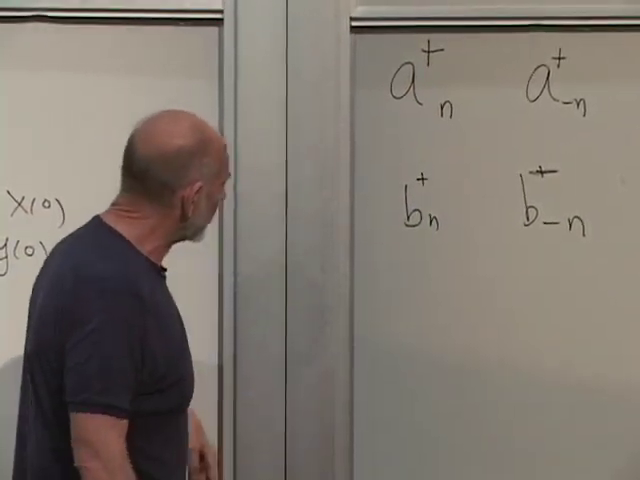
\includegraphics[width=0.65\textwidth]{lecture_04_figure_06.png}
  \caption{黑板记号中加倍后的\(X\)极化和\(Y\)极化产生算符。}
  \lectureframe{00:29:10}
  \label{fig:l04-oscillators-board}
\end{figure}

如果\(N_n^{(a)},N_n^{(b)}\)及其带波浪号的伙伴是占据数，那么两个方向上携带的振子能级示意为
\begin{equation}
  \begin{aligned}
    N&=\sum_{n>0}n\bigl(N_n^{(a)}+N_n^{(b)}+\cdots\bigr),\\
    \widetilde N&=\sum_{n>0}n
      \bigl(\widetilde N_n^{(a)}+\widetilde N_n^{(b)}+\cdots\bigr).
  \end{aligned}
  \label{eq:l04-level-operators}
\end{equation}
省略号表示额外的横向方向。

\section{失败的谱猜测}

回忆开弦的第一能级。用\(a_1^\dagger\)或\(b_1^\dagger\)作用于基态，给出两个线偏振。它们的圆组合，
\begin{equation}
  c_\pm^\dagger
  =
  \frac{1}{\sqrt2}
  \left(a_1^\dagger\pm i b_1^\dagger\right),
  \label{eq:l04-open-circular}
\end{equation}
携带螺旋度\(h=\pm1\)。没有螺旋度为零的伙伴，正是在这个初等四维描述中无质量矢量的标志。

设闭弦基态的质量平方为\(m_0^2\)。第一个朴素的猜测是用
\begin{equation}
  a_1^\dagger,\quad b_1^\dagger,\quad
  \widetilde a_1^\dagger,\quad\widetilde b_1^\dagger.
  \label{eq:l04-naive-one-sided}
\end{equation}
中的任意一个作用一次。这类似于开弦光子的两个副本，每个传播方向一个。然而在下一个能量级，不受限制的列表并不能组装成合理的转动多重态。更精细的记账并不能修复这个问题。认为每个振子单项式都是物理态这一前提是错误的。

\subsection{能级匹配，首先作为一条规则}

物理的闭弦条件是
\begin{equation}
  N=\widetilde N,
  \qquad\text{equivalently}\qquad E_L=E_R.
  \label{eq:l04-level-matching}
\end{equation}
目前先把它当作一个假设；只有在看到它达成了什么之后，才会推导它的起源。

\eqref{eq:l04-naive-one-sided}中的每个态在一个扇区中具有一份能量单位，而在另一个扇区中没有能量单位，因此每一个都被排除。最先存活下来的态从每一族中携带一个振子：
\begin{align}
  a_1^\dagger\widetilde a_1^\dagger\ket{0},
  &\qquad
  b_1^\dagger\widetilde b_1^\dagger\ket{0},
  \label{eq:l04-four-matched-a}\\
  a_1^\dagger\widetilde b_1^\dagger\ket{0},
  &\qquad
  b_1^\dagger\widetilde a_1^\dagger\ket{0}.
  \label{eq:l04-four-matched-b}
\end{align}
它们具有总振子能量二，在两个方向之间均分。单个\(n=2\)产生算符具有相同的总振子能量，但不满足\eqref{eq:l04-level-matching}；它只向一侧贡献两份能量单位。

\begin{figure}[H]
  \centering
  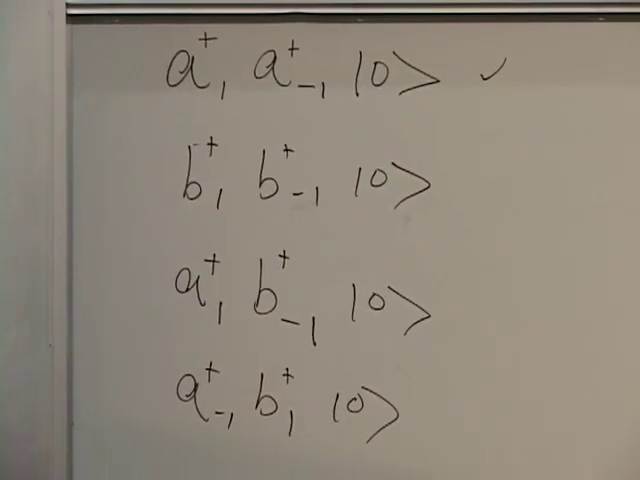
\includegraphics[width=0.70\textwidth]{lecture_04_figure_07.png}
  \caption{存活下来并通过能级匹配的四个第一能级态。图中使用下标\(1\)和\(-1\)，而\eqref{eq:l04-four-matched-a}--\eqref{eq:l04-four-matched-b}使用无波浪号和有波浪号的算符。}
  \lectureframe{00:41:05}
  \label{fig:l04-level-matched-board}
\end{figure}

\section{第一匹配能级中的引力子}

将两个手征族放入圆基：
\begin{equation}
  c_\pm^\dagger
  =\frac{a_1^\dagger\pm i b_1^\dagger}{\sqrt2},
  \qquad
  \widetilde c_\pm^\dagger
  =\frac{\widetilde a_1^\dagger\pm i\widetilde b_1^\dagger}{\sqrt2}.
  \label{eq:l04-closed-circular}
\end{equation}
每个因子在普通横向空间中贡献螺旋度\(+1\)或\(-1\)。因此它们的乘积给出
\begin{center}
\begin{tabular}{c c}
  \toprule
  态&螺旋度\\
  \midrule
  \(c_+^\dagger\widetilde c_+^\dagger\ket0\) & \(+2\) \\
  \(c_-^\dagger\widetilde c_-^\dagger\ket0\) & \(-2\) \\
  \(c_+^\dagger\widetilde c_-^\dagger\ket0\) & \(0\) \\
  \(c_-^\dagger\widetilde c_+^\dagger\ket0\) & \(0\) \\
  \bottomrule
\end{tabular}
\end{center}

\begin{classroomqa}
\audiencequestion{第二个圆偏振因子是否应来自相反的传播扇区？\lecturetimestamp{00:43:20}}
\lecturerresponse{是的。黑板上写下的第一个表达式正是因为这个原因而被更正。这里的物理态必须将一个右行振子与一个左行振子配对；否则它就不是能级匹配的。螺旋度指的是横向空间偏振，而这两个因子指的是相反的世界面方向。}
\end{classroomqa}

\begin{figure}[H]
  \centering
  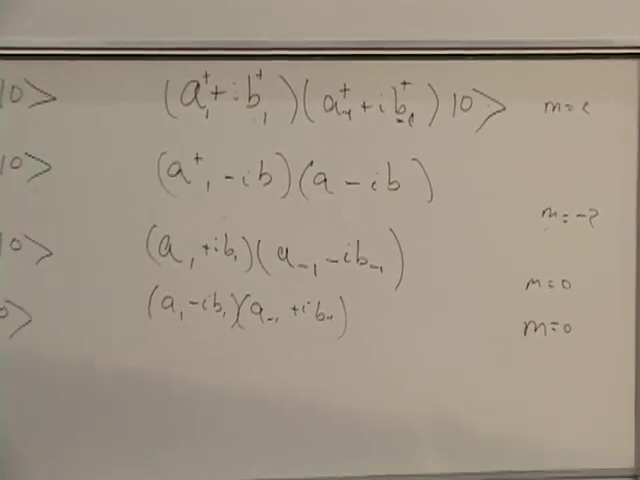
\includegraphics[width=0.82\textwidth]{lecture_04_figure_08.png}
  \caption{黑板更正后的四个圆基乘积，其螺旋度为\(+2,-2,0,0\)。}
  \lectureframe{00:46:10}
  \label{fig:l04-helicity-board}
\end{figure}

有质量的自旋二粒子有五个自旋投影，
\begin{equation}
  m=2,1,0,-1,-2.
\end{equation}
匹配能级不包含\(m=\pm1\)伙伴。因此它不可能是有质量的自旋二多重态。相比之下，无质量的自旋二粒子只有螺旋度\(+2\)和\(-2\)。同螺旋度乘积恰好就是这两个态：它们就是引力子偏振。

还剩下两个螺旋度为零的组合。用课上使用的语言来说，一个是膨胀子，另一个是轴子。对一般闭玻色弦的协变描述细化了这一陈述：
\begin{equation}
  \begin{aligned}
    \alpha_{-1}^{I}\widetilde\alpha_{-1}^{J}\ket{0;k}
    &\longrightarrow
    \underbrace{h_{IJ}}_{\text{symmetric traceless}}
    \oplus
    \underbrace{B_{IJ}}_{\text{antisymmetric}}\\
    &\hspace{2.5em}\oplus
    \underbrace{\Phi}_{\text{trace}}.
  \end{aligned}
  \label{eq:l04-massless-tensor-decomposition}
\end{equation}
这些是引力子、反对称二形式和膨胀子。在四维中，二形式可以对偶化为类轴子赝标量，这就是讲座中采用的语言。\editorialnote{第二个螺旋度为零的态在一般闭弦谱中从根本上就是反对称张量场\(B_{\mu\nu}\)。称其为轴子是四维对偶描述。}

在这个形式层面上，这三个场是无质量的。紧致化、投影和背景动力学可以改变哪些标量或二形式自由度保持轻。引力子则不同：一旦存在一个自洽的相互作用闭弦扇区，其无质量自旋二态就是不可避免的。这就是为什么引力从闭弦中涌现，而不是作为单独的成分被附加进去。

\section{为什么能级必须匹配}

我们现在回到\(\sigma=0\)处的标记。它是附着在圈上的物理珠子，还是仅仅是我们参数的起点？对于一条普通的无标记闭弦，不应有任何点享有特权。当所有标签一起平移时，量子态必须保持不变。

\subsection{离散版本}

将圈正则化为\(M\)个有序点，其横向坐标为\((X_i,Y_i)\)。暂时抑制\(Y_i\)。一个位形空间波函数是
\begin{equation}
  \Psi(X_1,X_2,\ldots,X_M).
\end{equation}
改变哪个点被称为第一个给出一个循环置换：
\begin{align}
  \Psi(X_1,X_2,\ldots,X_M)
  &=
  \Psi(X_2,\ldots,X_M,X_1)\nonumber\\
  &=
  \Psi(X_3,\ldots,X_M,X_1,X_2).
  \label{eq:l04-cyclic-wavefunction}
\end{align}
这不是在任意置换下的不变性。例如，在\(X_1\)和\(X_2\)之间插入\(X_3\)会改变邻接结构，并有效地撕裂和重新连接离散化的弦。只有共同的循环重标记
\begin{equation}
  X_i\longrightarrow X_{i+1}\qquad(\text{mod }M)
  \label{eq:l04-discrete-shift}
\end{equation}
表达了不存在优先起点。

\begin{figure}[H]
  \centering
  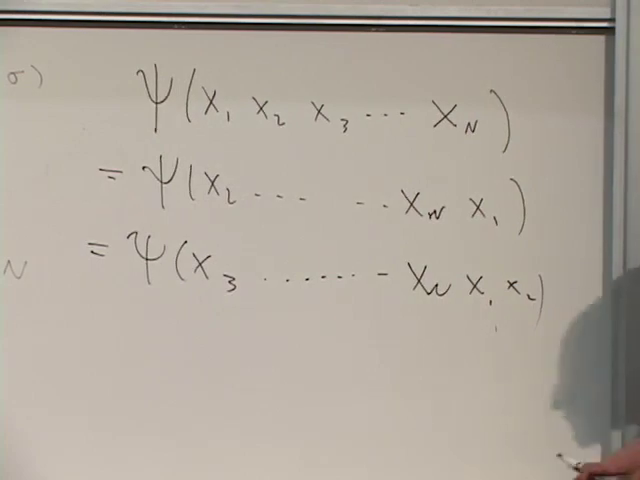
\includegraphics[width=0.82\textwidth]{lecture_04_figure_09.png}
  \caption{离散化闭弦的循环波函数恒等式。}
  \lectureframe{00:56:20}
  \label{fig:l04-cyclic-board}
\end{figure}

\subsection{连续版本}

在连续极限\(M\to\infty\)下，态是波泛函
\begin{equation*}
  \Psi[X(\sigma),Y(\sigma)].
\end{equation*}
循环重标记变为
\begin{equation}
  \sigma\longrightarrow\sigma+\epsilon.
\end{equation}
不变性表明
\begin{equation}
  \Psi[X(\sigma+\epsilon),Y(\sigma+\epsilon)]
  =
  \Psi[X(\sigma),Y(\sigma)].
  \label{eq:l04-wavefunctional-invariance}
\end{equation}

\begin{figure}[H]
  \centering
  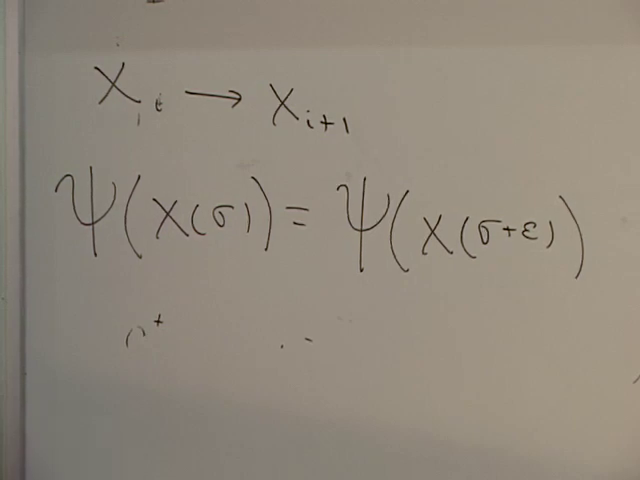
\includegraphics[width=0.72\textwidth]{lecture_04_figure_10.png}
  \caption{离散平移及其波泛函连续形式。}
  \lectureframe{00:58:40}
  \label{fig:l04-wavefunctional-board}
\end{figure}

在一阶近似下，
\begin{equation}
  \delta X(\sigma)=\epsilon X'(\sigma),
  \qquad
  \delta Y(\sigma)=\epsilon Y'(\sigma),
  \label{eq:l04-profile-shift}
\end{equation}
直到区分剖面的主动平移与坐标的被动平移的那个整体符号。相应的波泛函变分为
\begin{equation}
  \delta\Psi
  =
  \epsilon\int_0^{2\pi}d\sigma
  \left[
    \frac{\delta\Psi}{\delta X(\sigma)}X'(\sigma)
    +
    \frac{\delta\Psi}{\delta Y(\sigma)}Y'(\sigma)
  \right].
  \label{eq:l04-functional-variation}
\end{equation}

\begin{figure}[H]
  \centering
  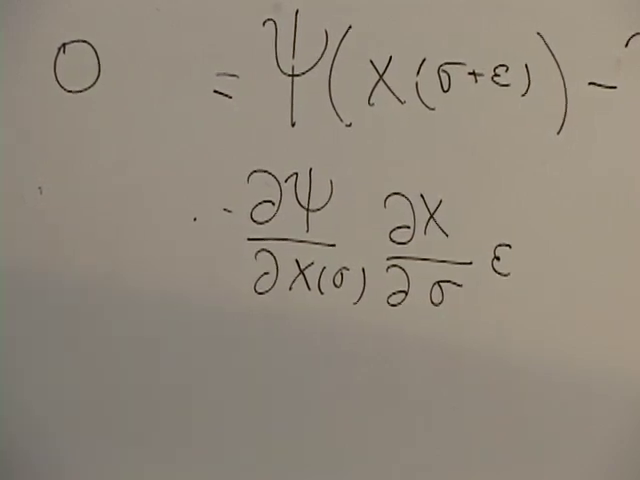
\includegraphics[width=0.72\textwidth]{lecture_04_figure_11.png}
  \caption{平移后波泛函自变量的一阶展开。}
  \lectureframe{01:01:31}
  \label{fig:l04-functional-expansion-board}
\end{figure}

\begin{classroomqa}
\audiencequestion{一阶条件是对\(\sigma\)的每一个值分别成立的独立方程吗？\lecturetimestamp{01:01:30}}
\lecturerresponse{不是。该变换将弦的每一点一起平移。某一点的变分必须与所有其他点的变分相加，这就是连续表达式包含对\(\sigma\)的积分的原因。}
\end{classroomqa}

在坐标表象中，
\begin{equation}
  P_X(\sigma)=-i\frac{\delta}{\delta X(\sigma)},
  \qquad
  P_Y(\sigma)=-i\frac{\delta}{\delta Y(\sigma)}
  \label{eq:l04-functional-momenta}
\end{equation}
其中\(\hbar=1\)。因此方程\eqref{eq:l04-functional-variation}由下式生成：
\begin{equation}
  G_\sigma=
  \int_0^{2\pi}d\sigma\,
  \left[
    P_X(\sigma)X'(\sigma)+P_Y(\sigma)Y'(\sigma)
  \right].
  \label{eq:l04-sigma-generator}
\end{equation}
这正是Noether模式\eqref{eq:l04-noether-charge}：正则动量乘以坐标位移，并对所有自由度求和。一个无标记的闭弦态满足
\begin{equation}
  G_\sigma\ket{\mathrm{phys}}=0.
  \label{eq:l04-physical-generator-condition}
\end{equation}

对于\eqref{eq:l04-string-lagrangian}的归一化，
\(P_I\propto\dot X^I\)，因此同一条件可写为
\begin{equation}
  \int_0^{2\pi}d\sigma
  \sum_I\dot X^I X^{I\prime}=0.
  \label{eq:l04-momentum-constraint}
\end{equation}

\begin{figure}[H]
  \centering
  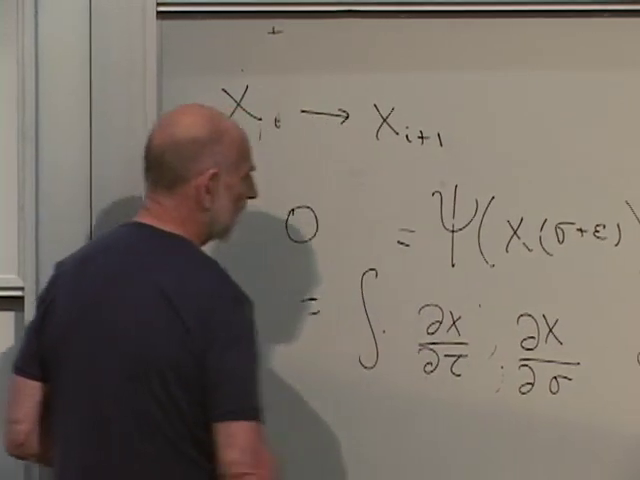
\includegraphics[width=0.75\textwidth]{lecture_04_figure_12.png}
  \caption{在波泛函的导数被等同于动量之后，积分后的生成元。}
  \lectureframe{01:05:10}
  \label{fig:l04-generator-board}
\end{figure}

\subsection{生成元是能量差}

\eqref{eq:l04-left-right-energies}中两个表达式之和是总能量。它们的差为
\begin{align}
  E_L-E_R
  &\propto
  \frac12\int_0^{2\pi}d\sigma\sum_I
  \left[
    (\dot X^I+X^{I\prime})^2\right.\nonumber\\[-0.25em]
  &\hspace{7em}\left.
    -(\dot X^I-X^{I\prime})^2
  \right]\\
  &=
  2\int_0^{2\pi}d\sigma\sum_I
  \dot X^I X^{I\prime}.
  \label{eq:l04-energy-difference}
\end{align}
该积分就是必须湮灭物理态的生成元。因此
\begin{equation}
  E_L-E_R=0,
  \qquad\text{or}\qquad
  N-\widetilde N=0.
\end{equation}
能级匹配所陈述的是：\(\sigma\)坐标的原点是不可观测的。

\begin{figure}[H]
  \centering
  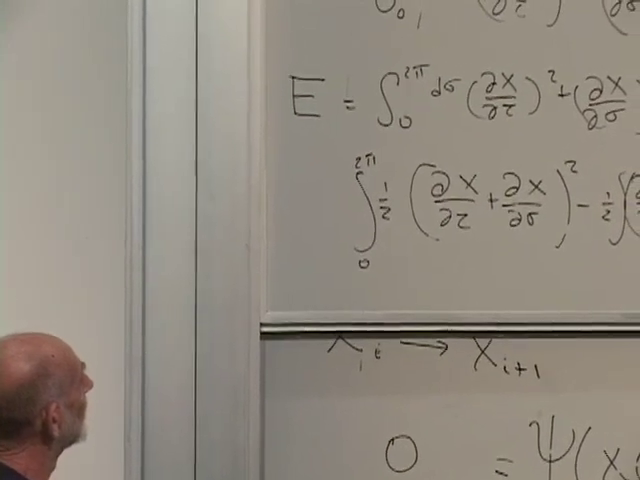
\includegraphics[width=0.78\textwidth]{lecture_04_figure_13.png}
  \caption{在能级匹配推导末尾一起展示的能量之和与能量之差。}
  \lectureframe{01:06:40}
  \label{fig:l04-energy-difference-board}
\end{figure}

\begin{classroomqa}
\audiencequestion{为什么这些展示的公式似乎把二分之一因子的位置放得不同？\lecturetimestamp{01:06:28}}
\lecturerresponse{这里只用到相对结构。恢复一个一致的整体归一化，就得到配平方恒等式\eqref{eq:l04-energy-square-completion}中的二分之一。求和给出总能量，而差值仍正比于
\(\int d\sigma\,\dot X X'\)。它的消失，从而能级匹配，与那个共同的约定无关。}
\end{classroomqa}

该约束去掉了朴素振子谱的很大一部分，而且恰好去掉了那些未能形成合理粒子多重态的态。它并不去掉开弦光子，因为开弦不具有两个受此闭弦回路条件约束的独立循环扇区。对于闭弦，它保留了引力子、膨胀子、反对称张量态或类轴子态，以及更高的匹配能级。
\editorialnote{在协变弦量子化中，能级匹配是零模条件\(L_0-\widetilde L_0=0\)，即世界面约束系统中的一个成员。这里的推导揭示了它的直观起源：闭弦绕圈平移下的不变性。}

\section{左与右的两种含义}

现在“手性”语言有两种互不相关的用法：
\begin{enumerate}
  \item \(X_R(\tau-\sigma)\)与\(X_L(\tau+\sigma)\)描述沿内禀\(\sigma\)圆朝相反方向的传播。
  \item \(c_+^\dagger\)与\(c_-^\dagger\)描述物理横向\(xy\)平面中的圆偏振。
\end{enumerate}
能级匹配的引力子态包含来自每个世界面方向的一个振子。然而这两个振子可以具有相同的时空螺旋度，从而产生\(h=+2\)或\(h=-2\)。混淆这两种左与右，会使谱看起来自相矛盾，而实际上并非如此。

\section{基本是什么意思？}

一旦开弦和闭弦在这个初等层面上被量子化，一个自然的问题仍然存在：弦是最终组分吗，还是它们本身也可能由别的东西构成？

\begin{classroomqa}
\audiencequestion{是否有证据或理由把弦视为最基本客体，其下没有更小的东西？\lecturetimestamp{01:10:44}}
\lecturerresponse{不存在有用的、与参数无关的答案。在某一区域看起来基本的自由度，在另一区域可能变得重、延展，并且显得像是复合的。最好把“基本”理解为关于在所考虑的耦合下哪些变量提供了有用描述的陈述。}
\end{classroomqa}

电荷与磁荷为这一答案提供了最干净的模型。假设一个理论包含电荷 \(e\) 和磁荷 \(g\)。附着在单极子上的不可观测的狄拉克弦要求
\begin{equation}
  eg=2\pi n,
  \qquad n\in\mathbb Z.
  \label{eq:l04-dirac-quantization}
\end{equation}
对于最小电荷，\(n=1\)。一个绕狄拉克弦运动的带电粒子随后获得相位 \(e^{ieg}=1\)，因此这条辅助弦无法被探测到。

\begin{figure}[H]
  \centering
  \begin{minipage}[t]{0.58\textwidth}
    \centering
    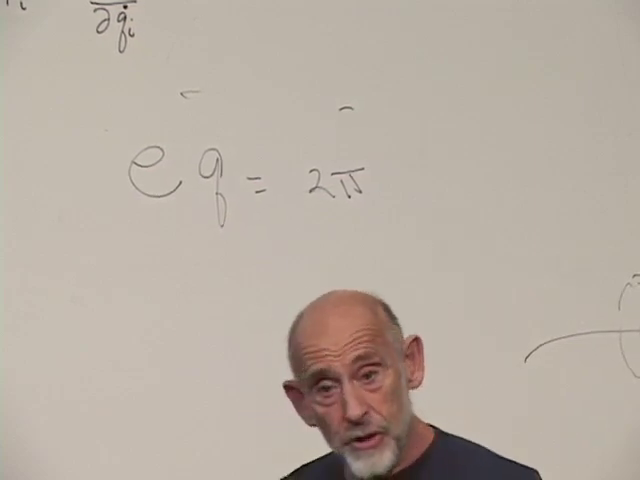
\includegraphics[width=\textwidth]{lecture_04_figure_14.png}
    \par\smallskip\footnotesize (a) 黑板上的狄拉克量子化。
  \end{minipage}\hfill
  \begin{minipage}[t]{0.36\textwidth}
    \centering
    \begin{adjustbox}{max width=\linewidth}
    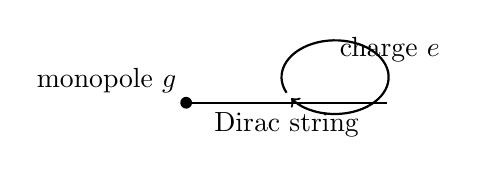
\begin{tikzpicture}[scale=0.85]
      \fill (0,0) circle (2.5pt);
      \node[above left] at (0,0) {monopole \(g\)};
      \draw[thick] (0,0) -- (3.0,0);
      \node[below] at (1.5,0) {Dirac string};
      \draw[->,thick] (1.5,0.15) arc[start angle=205,end angle=-145,
        x radius=0.8,y radius=0.55];
      \node[right] at (2.15,0.8) {charge \(e\)};
    \end{tikzpicture}
    \end{adjustbox}
    \par\smallskip\footnotesize (b) 围绕弦的相位实验。
  \end{minipage}
  \caption{电荷与磁荷通过狄拉克条件成反比关系。}
  \lectureframe{01:13:20}
  \label{fig:l04-dirac-board}
\end{figure}

如果 \(e\) 很小，则以电变量进行的普通微扰论是有用的。带有额外电顶点的费曼图受到越来越强的压低。但 \eqref{eq:l04-dirac-quantization} 随后使 \(g\) 变大，因此以磁顶点进行的图解展开并不有用。用通常的无量纲耦合常数表示，
\begin{equation}
  \alpha_e=\frac{e^2}{4\pi},
  \qquad
  \alpha_m=\frac{g^2}{4\pi},
  \qquad
  \alpha_e\alpha_m=\frac{n^2}{4}.
  \label{eq:l04-dual-couplings}
\end{equation}
弱电耦合就是强磁耦合，反之亦然。

强耦合的单极子从电的描述来看也显得复杂。它的场能很大；它被强烈的规范场涨落云和虚的带磁荷对所包裹。它表现为一个沉重的、延展的客体，是电微扰级数的一个糟糕出发点。这并不证明它不那么基本。它只是说，对于那个区域而言，它是错误的初等变量。

现在想象连续增大 \(e\)。量子化条件迫使 \(g\) 减小。在自对偶区域附近，两种描述都不特别弱，而越过该区域后，磁变量可以成为更简单、更轻的变量，而电客体则变得被强烈包裹。哪个电荷应被称为基本电荷已经改变，而理论的物理内容并未改变。

\subsection{维格纳之问}

这一模糊性曾在关于希格斯玻色子是基本的还是复合的讨论中浮现出来。尤金·维格纳反复追问复合意味着什么。一个被提出的区分是衰变：也许基本客体不能衰变，而复合客体可以。但基态氢原子不能衰变，却显然是复合的；质子可能稳定而中子衰变，然而这并不使其中一个成为基本的、另一个成为所意指意义上的复合的。每一个简单的定义都产生了另一个反例。

赫拉尔杜斯·特霍夫特以操作性的判据结束了讨论：当一个客体把它想成基本的很有用时，它就是基本的。这不是回避。它承认，基本一词标识的是动力学在其中简单的那些变量，而简单性可以依赖于耦合和环境。

\section{走向M理论}

弦理论以特别鲜明的方式实现了这种角色的交换。在一个参数区域中，弦是轻的且是微扰的，而D膜看起来像是由弦自由度构成的沉重孤子式复合体。随着参数变化，D膜可以成为更轻的基本客体，而在第一个区域中被描述为弦的位形可以用它们来重新解释。看起来基本的可以变成复合的；看起来复合的可以变成基本的。

旧的还原论图景暗示着从大的事物到更小的组分、最终到唯一底层的一种单向下降。对偶性暗示着某种不那么线性的东西：描述可以随着耦合变化而相互转化，没有任何单一组变量在所有地方都享有特权。这正是接近下一个主题——M理论——的视角。

为什么玻色弦的临界维数是二十六、超弦的临界维数是十，这些问题在此仍然悬而未决。与其在继续前进之前解决每一个技术问题，我们现在改变视角，追问M理论如何能在适当的极限下产生弦理论。
